% !TEX TS-program = pdflatex
% !TEX encoding = UTF-8 Unicode

% This is a simple template for a LaTeX document using the "article" class.
% See "book", "report", "letter" for other types of document.

\documentclass[11pt]{report} % use larger type; default would be 10pt

\usepackage[utf8]{inputenc} % set input encoding (not needed with XeLaTeX)
\usepackage[T1]{fontenc}

%%% Examples of Article customizations
% These packages are optional, depending whether you want the features they provide.
% See the LaTeX Companion or other references for full information.

%%% PAGE DIMENSIONS
\usepackage{geometry} % to change the page dimensions
\geometry{a4paper} % or letterpaper (US) or a5paper or....
% \geometry{margin=2in} % for example, change the margins to 2 inches all round
% \geometry{landscape} % set up the page for landscape
%   read geometry.pdf for detailed page layout information

\usepackage{graphicx} % support the \includegraphics command and options

% \usepackage[parfill]{parskip} % Activate to begin paragraphs with an empty line rather than an indent

%%% PACKAGES
\usepackage{booktabs} % for much better looking tables
\usepackage{array} % for better arrays (eg matrices) in maths
\usepackage{paralist} % very flexible & customisable lists (eg. enumerate/itemize, etc.)
\usepackage{verbatim} % adds environment for commenting out blocks of text & for better verbatim
\usepackage{subfig} % make it possible to include more than one captioned figure/table in a single float
\usepackage{pgfgantt} % diagram of gantt
\usepackage[francais]{babel}
% These packages are all incorporated in the memoir class to one degree or another...

%%% HEADERS & FOOTERS
\usepackage{fancyhdr} % This should be set AFTER setting up the page geometry
\pagestyle{fancy} % options: empty , plain , fancy
\renewcommand{\headrulewidth}{1pt} % customise the layout...
\lhead{WebMedia Manager}\chead{}\rhead{\leftmark}
\renewcommand{\footrulewidth}{1pt} % customise the layout...
\lfoot{Jean-Philippe Froelicher}\cfoot{\thepage}\rfoot{\today}

% other preamble stuff...
\usepackage{etoolbox}
\patchcmd{\chapter}{\thispagestyle{plain}}{\thispagestyle{fancy}}{}{}

%%% SECTION TITLE APPEARANCE
\usepackage{sectsty}
\allsectionsfont{\sffamily\mdseries\upshape} % (See the fntguide.pdf for font help)
% (This matches ConTeXt defaults)

%%% ToC (table of contents) APPEARANCE
\usepackage[nottoc,notlof,notlot]{tocbibind} % Put the bibliography in the ToC
\usepackage[titles,subfigure]{tocloft} % Alter the style of the Table of Contents
\renewcommand{\cftsecfont}{\rmfamily\mdseries\upshape}
\renewcommand{\cftsecpagefont}{\rmfamily\mdseries\upshape} % No bold!

%$HeadURL: https://subversion.assembla.com/svn/cfpt-courses/trunk/_inc/inc_lst_csharp.tex $
%$LastChangedDate: 2014-01-22 11:03:53 +0100 (mer., 22 janv. 2014) $
%$LastChangedRevision: 5197 $
%$LastChangedBy: marechal $

% lstlisting configuration for C#
%-------------------------------------------------------------------------------------
\usepackage{xcolor}
\usepackage{listings}
\usepackage{accsupp}

% color
\definecolor{lightgreen}{rgb}	{0.200, 0.980, 0.200}
\definecolor{darkgreen}{rgb}	{0.000, 0.400, 0.000}
\definecolor{lightgray}{gray}	{0.98}
\definecolor{darkred}{rgb}		{0.545, 0.000, 0.000}

% CSharp colors
\definecolor{class}{rgb}		{0.200, 0.600, 0.600}	% Cyan Visual Studio
\definecolor{keyword}{rgb}		{0.000, 0.000, 1.000}	% blue

% code to avoid line number copy during copy-paste from PDF
\newcommand{\noncopynumber}[1]{%
    \BeginAccSupp{method=escape,ActualText={}}%
    {\scriptsize#1}%
    \EndAccSupp{}%
}

% lstlisting parameters
\lstset {	
  language=[Sharp]C
, captionpos=b
, frame=shadowbox
, rulesepcolor=\color{gray}
% syntaxic coloration
, basicstyle=\footnotesize\ttfamily
, keywordstyle=\color{blue}
, commentstyle=\color{darkgreen}
, stringstyle=\color{darkred}
, backgroundcolor=\color{lightgray}
, identifierstyle=\color{black}
% lines numbering
, numbers=left
, numberstyle=\noncopynumber
, stepnumber=1
, numbersep=5pt
%
, breaklines=true
, tabsize=2
, showstringspaces=false
, lineskip={-1.5pt} % single line spacing
, escapeinside={/*(*@}{@*)*/}
, rangeprefix=\{\  % curly left brace plus space
, rangesuffix=\ \} % space plus curly right brace
}

% Csharp : additional keywords
\lstset{
	morekeywords={var,get,set,string,value},
	otherkeywords={\#region,\#endregion,\#define,\#if,\#endif,\#else}, %morekeyword does not support # chararacter then we must use otherkeywords
	emph={[1]Application,
		Char,Color,Console,Convert,
		DialogResult,
		Environment,EventArgs,
		Form,
		Object,String,
		SByte,Int16,Int32,Int64,
		Byte,UInt16,UInt32,UInt64,
		Single,Double,
		Keys,KeyPressEventArgs,
		MessageBox,MessageBoxButtons},
	emphstyle={[1]\color{class}}
}

\lstset{prebreak=\raisebox{0ex}[0ex][0ex]
        {\ensuremath{\hookleftarrow}}}
%\lstset{postbreak=\raisebox{0ex}[0ex][0ex]
%        {\ensuremath{\hookrightarrow\space}}}
\lstset{breaklines=true, breakatwhitespace=true}

% replace sequence of char by another sequence of char
% see http://stackoverflow.com/questions/1116266/listings-in-latex-with-utf-8-or-at-least-german-umlauts
\lstset{literate=%
{ä}{{\"a}}1
{â}{{\^a}}1
{à}{{\`a}}1
{Ä}{{\"A}}1
{Â}{{\^A}}1
{À}{{\`A}}1
{ë}{{\"e}}1
{ê}{{\^e}}1
{é}{{\'e}}1
{è}{{\`e}}1
{Ë}{{\"E}}1
{Ê}{{\^E}}1
{É}{{\'E}}1
{È}{{\`E}}1
{ï}{{\"i}}1
{î}{{\^i}}1
{Ï}{{\"I}}1
{Î}{{\^I}}1
{ö}{{\"o}}1
{ô}{{\^o}}1
{Ö}{{\"O}}1
{Ô}{{\^O}}1
{ü}{{\"u}}1
{û}{{\^u}}1
{ù}{{\`u}}1
{Ü}{{\"U}}1
{Û}{{\^U}}1
{Ù}{{\`U}}1
{ç}{{\c c}}1
{Ç}{{\c C}}1
{°}{{\textsuperscript{o}}}1
% suppress BOM (Byte Order Mark) characters at the beginning of Visual Studio source
% see http://tex.stackexchange.com/questions/5935/how-to-suppress-bom-effect-in-the-output
{�}{}0
{�}{}0
{�}{}0
}



%%% END Article customizations

%%% The "real" document content comes below...

\title{Web Media Manager}
\author{The Author}
%\date{} % Activate to display a given date or no date (if empty),
         % otherwise the current date is printed 

\begin{document}
	
\maketitle
\newpage

\tableofcontents

\chapter{Résumés}

\chapter{Introduction}

\chapter{Cahier des charges}
	\section{Titre du projet}
	WebMedia Manager

	\section{Objectifs du projet}
	Création d’une application permettant l’utilisation des différents services proposés par les sites de vidéos et de diffusion de flux vidéo en direct.
	Les fonctions de bases liées au services en question sont intégrées génériquement dans l’application.
	Des fonctions ajoutées par moi-même y sont également ajoutées.
	L’application a pour but de faciliter l’utilisation de ses services pour les utilisateurs ayant une fréquentation régulière de ceux-ci.

	\section{Description détaillée}
	L’application propose un certains nombre de service lié à la plateforme d’hébergement et de diffusion des vidéos. En effet, plusieurs sites vidéo comme Youtube, Dailymotion, Twitch etc. propose des services de bases pour leurs utilisateurs.
	Elle reprend si possible dynamiquement les différentes fonctions de chaque site et les proposes dans une interface crée à cet effet.

	Les fonctions de bases que l’application propose pour chaque site :
	\begin{itemize}
		\item Connexion avec un compte lié au site, donc créer auparavant ;
		\item Modification des différents paramètres de comptes ;
		\item Recherches de flux vidéos suivant différents critères : Nom d’un flux vidéo, nom du jeux, nom d’une chaîne, nom d’un utilisateur etc ;
		\item Affichage d’une vidéo ou d’une diffusion en direct ;
		\item La fonction "Suivre" ou "S’abonner" qui consiste à être mis au courant des nouvelles vidéos / diffusion ;
		\item Affichage détaillé d’un utilisateur : Accès à ses informations publique, ses vidéos etc ;
		\item Affichage des vidéos / diffusions en direct les plus populaires ;
		\item Affichage de l’espace communautaire : Commentaire vidéos, Chat sur une diffusion en direct
	\end{itemize}
	
	Les fonctions ci-dessus sont celle de base pour chaque sites à quelques exception près.
	
	Ci-dessous, les fonctions ajoutée par moi-même dans l’application :
	\begin{itemize}
		\item Système de notification lorsqu’une vidéo sort ou qu’une diffusion en direct commence ;
		\item Création de catégorie pour organiser les différents flux vidéos suivis, les catégories sont inter-services, c'est-à-dire que l’on peut mélanger les différents contenu des sites.
		\item Création de playlist pour lire plusieurs vidéos à la suite, également inter-services. Par contre cela ne s'applique uniquement sur les vidéos, on ne peut pas créer de playlist de diffusion en direct.
	\end{itemize}

	Pour la réalisation de cette application j’utilise le langage C\#.

	\section{Inventaire des étapes}
	Début : Lundi 13/04/2015 \\
	Reddition intermédiaire (doc + poster) : Vendredi 30/04/2015 \\
	Reddition finale : Lundi 01/06/2015
	
	\section{Inventaire du matériel}
	PC + 2 écrans

	\section{Inventaire des logiciels}
	Visual Studio 2013 Professionnel
	
	\section{Délivrables (documents à restituer)}
	\begin{itemize}
		\item 1 journal de bord (format A5)
		\item 1 poster A2
		\item 2 exemplaires papier de la documentation technique
		\item 2 exemplaires papier du mode d'emploi (si besoin)
		\item 1 CD/DVD ROM contenant tous les fichiers (sources + documentation + poster)
		\item Une démonstration fonctionnelle du projet, une solution parmi :
		\begin{itemize}
			\item live CD, live USB
			\item machine virtuelle (VirtualBox) pré-configurée
		\end{itemize}
	\end{itemize}

	\section{Éléments mesurables (servant à l'évaluation)}
	Réalisation des objectifs, mesurées selon la grille d'évaluation.

\chapter{Étude d'opportunité}
	\section{Introduction au projet}
	Le but de ce projet est de réaliser une application permettant l'utilisation des différents services proposé par les sites de vidéos et de diffusion de flux vidéo en direct.
		\subsection{Médias vidéo web}
		 Aujourd'hui, les sites comme Youtube, Dailymotion, Twitch qui propose du contenu vidéos sont de plus en plus visités. Ses sites, ont tous un point commun, d'autres personnes mettent des vidéos en ligne pour divertir les spectateurs. \\
		 Le phénomène a prit une tel ampleur que certain "créateur de contenu audiovisuel" sont même payé par ses sites par rapport à leur popularité. De plus en plus de personnes, surtout les jeunes, passent leurs temps devant des vidéos sur le web que sur la télévision.
			\subsubsection{Direct}
			Les vidéos en direct sont de plus en plus présent sur le web. En effet, grâce en grande partie aux jeux vidéos, le phénomène des personnes créant du contenu audiovisuel c'est également répandu sur du contenu en direct. Des sites comme Twitch ou Dailymotion propose à ses utilisateurs de diffuser du flux vidéo en direct. \\ 
			La plus part du temps c'est pour les jeux vidéos, les diffuseurs jouent sur leurs ordinateurs / consoles puis, retransmet l'image sur le site. Ainsi, des personnes du monde entier ont la possibilité de regarder la partie de jeu d'une personne. Les spectateurs ont même la possibilité de discuter avec les autres spectateurs et même des fois avec le diffuseur de contenu.\\
			Les diffuseurs sont payés grâce aux dons de leurs communauté, certain font ça à plein temps et donc sont contraint à entretenir une grande communauté.
			\subsubsection{Différé}
			Les vidéos "différé" sont depuis un petit moment déjà présente sur le web. En effet, le phénomène des vidéos sur le web n'est pas tout nouveau mais, ce n'est que depuis peu que le phénomène à prit une grande ampleur. \\
			Si un créateur de contenu à atteint une certaine popularité, il peut enfin prétendre à faire de l'argent avec ses vidéos. En effet, le premier site de vidéos du monde Youtube rémunère les créateurs de contenu.

		\subsection{Pourquoi avoir choisi ce sujet ?}
		J'ai choisi ce sujet car je porte un réel intérêt au monde audiovisuel sur le web. En effet, je fais parti des jeunes qui a délaissé la télévision pour les vidéos sur internet. Il y a plusieurs site de vidéos et souvent il est difficile de s'y retrouver, l'application que j'ai pensé a pour but de faciliter la vie des personnes comme moi qui utilise ses sites régulièrement. Le fait que le monde de l'audiovisuel est en plein boum sur le web me stimule encore plus à l'idée de créer une application dans ce domaine. \\
		On retrouve également de plus en plus de site proposant à ses utilisateurs de pouvoir diffuser du flux vidéo en direct, ce qui consolide l'intérêt de mon application.

	\section{Analyse de l'existant}
	Il n'y a pas d'application similaire à celle que je vais réaliser. Tout de même, les différentes fonctions que je veux y intégrée sont déjà présente sur les différents sites.
		\subsection{Existant}
		\begin{itemize}
			\item Twitch now : Application Google Chrome
			\item Dailymotion Games : Application Android
		\end{itemize}			
		\subsection{Critique de l'existant}	
		\textbf{Twitch now} : Cette application permet à l'utilisateur de naviguer dans les différentes diffusion de flux vidéo en direct de Twitch. C'est une application Google Chrome, elle permet de naviguer sur Twitch sans aller sur le site. Le système de "suivis" est celui de Twitch, c'est-à-dire qu'il faut se connecter avec son propre compte Twitch.
		
		\textbf{Dailymotion Games} : Cette application permet aux utilisateurs de Dailymotion de naviguer entre les différentes diffusion de flux vidéo en direct. Par contre, on ne peut pas se connecter à son compte personnel pour avoir uniquement que les diffusions que l'on est abonné. Les différentes diffusion sont classé soit par vues, soit par jeux. Évidemment, les diffusions de flux vidéo peuvent être visionnée depuis l'application.
		Dailymotion Games est une application officiel de Dailymotion.
		
		
\chapter{Analyse fonctionnelle}
	\section{Description du fonctionnement}
		\subsection{Fonctions des sites}
			\subsubsection{Générique}
			Tout les sites proposent des fonctions "commune" de base qui sont intégrée à WebMedia Manager:
			\begin{itemize}
				\item Affichage des dernières vidéos / diffusion en direct
				\item Recherche une vidéo / diffusion en direct
				\item Affichage d'une vidéo / diffusion en direct
				\item Connexion au service en question
				\item Modification des paramètres du compte connecté
				\item Afficher les détails d'un utilisateur
				\item Afficher les vidéos / diffusion en direct populaire
				\item Gestion des notifications
				\item Suivre une chaîne / un utilisateur
			\end{itemize}
			
			\subsubsection{Diffusion en direct}
			Les fonctions spécifique aux sites qui proposes des diffusions en direct :
			\begin{itemize}
				\item \textit{Chat} : Discuter avec les autres spectateurs
				\item Abonnement payant
			\end{itemize}
			Les utilisateurs ont le la possibilité de faire des donations mais pas par le biais des sites de diffusions.
			
			\subsubsection{Vidéo en différé}
			Les fonctions spécifique aux sites qui proposes des vidéos en différé :
			\begin{itemize}
				\item Commentaires : Donner un avis / discuter avec les autres spectateurs
			\end{itemize}
	
		\subsection{Gestion des catégories}
		Les catégories servent à rassembler plusieurs vidéos de différents sites. En effet, grâce aux catégories, les vidéos peuvent être organiser même si elles ne viennent pas du même site.
		
		Action possible sur une catégorie :
		\begin{itemize}
			\item Ajouter
			\item Modifier le nom
			\item Supprimer
		\end{itemize}
		
		La seule action possible sur une vidéo est de la supprimer.
		
		\subsection{Gestion des listes de lecture}
		Les listes de lecture servent à lire un certain nombre de vidéo à la suite. Les listes de lectures sont également inter-site.
		
		Action possible sur une liste de lecture :
		\begin{itemize}
			\item Ajouter
			\item Modifier le nom
			\item Supprimer
		\end{itemize}
		
		Actions possible sur une vidéo :
		\begin{itemize}
			\item Supprimer
			\item Monter (dans la liste)
			\item Descendre (dans la liste)
			\item Déplacer à X position (dans la liste)
		\end{itemize}
		
		\subsection{Notifications}
		Les notification servent à être tenu au courant lors de nouvelle diffusion en direct ou lorsqu'une nouvelle vidéo sort.
		Lorsque un utilisateur suit un auteur de vidéo, il sera de toute façon notifié.
		L'application donne la possibilité à l'utilisateur d'activé ou de désactiver les notifications.
		
		
		
	\section{API}
	Les API des différents site permettent de faire des interrogations entre les bases de données et l'application.
		\subsection{API REST}
		Les API\footnote{Application Programming Interface} REST\footnote{Representational State Transfer} servent à accéder a une ressource par son URI grâce au protocole HTML pour procéder à diverses opérations : GET; POST; PUT; DELETE. \\		
		Le format de représentation des données est libre, dans le cas des API que l'on utilise, le format est en JSON\footnote{JavaScript Object Notation}.
		
		\begin{figure}[h]
			\center
			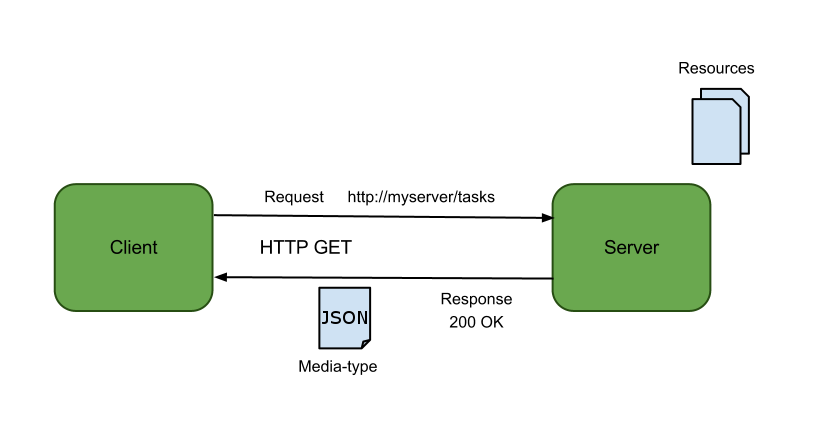
\includegraphics[width=0.9\textwidth]{../img/rest.png}
			\caption{REST}
			\label{rest}
		\end{figure}
		
		\noindent
		Les ressources sont accessible via les liens que l'API met à disposition :

		\begin{itemize}
		\item https://api.dailymotion.com : pour le site Dailymotion
		\item https://api.twitch.tv : pour le site Twitch
		\item https://api.vimeo.com : pour le site Vimeo
		\end{itemize}
		
		Toutes ses API mettent à disposition des URL qui servent à récupérer des ressources précises. 
		
		
	\section{Lecteur vidéo}
	Afin d'afficher le flux vidéo des différentes vidéos ou des différente diffusion en direct, les sites ont leurs propre lecteur vidéo.
	Ils se présentent généralement sous un format \textit{Flash player} ou HTML5.
	
		\subsection{Flash player}
		Le plus part des sites utilisent le lecteur flash pour leurs lecteurs vidéo. Le lecteur flash utilise le protocole RTMP\footnote{Real Time Messaging Protocol}, c'est un protocole réseau propriétaire développé par Adobe Systems. Il sert à la diffusion de flux de données en streaming(audio, vidéo ...) entre un serveur et un client.
		
		\subsection{HTML5}
		Un nouveau format de lecteur vidéo est apparu sur le web depuis peu, il s'agit du lecteur HTML5. Ce lecteur utilise un autre codec (VP9), le codec libre de Google qui compresse la vidéo. Ce codec a été mis en place surtout pour accélérer l'accession au contenu HD 4k à 60 fps\footnote{Frame Per Second}.
		Le fait d'utiliser le lecteur HTML5 est un plus dans le multi-plateforme.
	
	\section{Outil communautaire}
	Les différents sites de vidéos mettent à disposition des utilisateurs des outils afin de pouvoir communiquer avec d'autre membre du site ou directement s'adresser à l'auteur de la vidéo.
		\subsection{Chat IRC}
		Le \textit{chat} est utilisé le plus souvent lors de diffusion de flux vidéo en direct. Afin d'avoir un contact direct avec le diffuseur il faut avoir un support sur lequel le diffuseur peut lire rapidement.
		
		La plus part des \textit{chat} utilisé pour les diffusions de flux vidéo en direct sont des \textit{chats} IRC\footnote{Internet Relay Chat}.
		
		IRC est un protocole de communication textuelle, il sert à la communication instantanée sous la forme de discussions de groupe par l'intermédiaire de canaux de discussion. Il peut également être utilisé pour communiquer de un à un.
		Le principe est que chaque utilisateur est connecté à un serveur IRC qui eux-même sont relié avec d'autres serveurs IRC. Ainsi toutes les personnes peuvent discuter sur des forums publics ou privé.
		
		Les différents site de diffusion en direct utilise le client IRC "Kiwiirc" conçue spécialement pour le web, cela ajoute au chat IRC plein de caractéristiques qui améliore l'utilisation du chat.
		
		\subsection{Commentaires}
		Les commentaires servent à discuter avec d'autre personne sur la vidéo en question. Ils servent également à communiquer avec l'auteur de la vidéo.
		Il n'y a pas de commentaire sur les diffusions de flux vidéo en direct.
		
	\newpage
	\section{Connexion}
	Afin de se connecter aux différents services avec un compte personnel, ils utilisent le protocole OAuth2.
		\subsection{OAuth2}
		La plus part des grands sites utilisent le protocole OAuth2 pour l'authentification au compte personnel, en effet, ce protocole permet d'obtenir un accès limité à un service via HTTP par le biais d'une autorisation. 
		La demande d'accès est demandée par le client, en l'occurrence WebMedia Manager.
	
		OAuth2 définit 4 rôles :
		\begin{itemize}
			\item Détenteur des données (L'utilisateur)
			\item Serveur de ressources (Twitch, Youtube, Dailymotion ...)
			\item Client (WebMedia Manager)
			\item Serveur d'autorisation (Twitch, Youtube, Dailymotion ...)
		\end{itemize}
		
			\subsubsection{Token (jeton)}
			Lorsque le client fait une demande d'authentification, le serveur d'autorisation délivre un token. Un token permet au serveur de ressources d'autoriser la mise à disposition des données d'un utilisateur. Il a une durée de vie limité qui est définie par le serveur qui délivre les tokens.
			Un token doit rester le plus confidentiel possible, même l'utilisateur ne voit pas son token attribué.
			
			\subsubsection{Scope (portée)}
			Le scope est un paramètre qui sert à définir les droits sur un token. En effet, le serveur d'autorisation propose une liste de scope et lors de l'authentification, attribut ses droits sur le token.
			
			\subsubsection{Type d'autorisation}
			Il existe deux types d'autorisation : Flux de code d'autorisation(\textit{Autorization Code Flow}) et l'autorisation implicite(\textit{Implicit Grant Flow}). L'autorisation implicite s'utilise quand l'application se trouve côté client. La demande d'authentification se fait de la sorte :
			\begin{enumerate}
				\item L'application souhaite accéder aux données
				\item Requête d'autorisation au serveur
				\item Si l'accès est autorisé, le serveur d'autorisation délivre le token
				\item Utilisation du token pour certaine requête 
			\end{enumerate}
			
			\newpage
			
			\begin{figure}[h]
				\center
				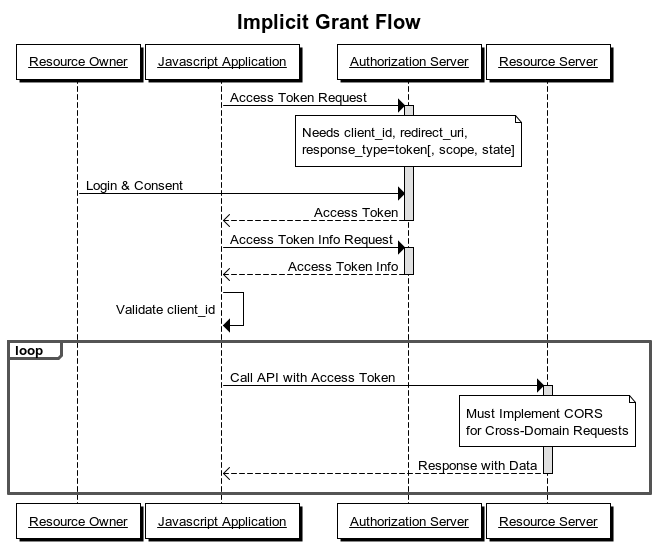
\includegraphics[width=1\textwidth]{../img/SchemaOAuth2.png}
				\caption{Schéma OAuth2 : Droit implicite}
				\label{oauth2}
			\end{figure}
			
			\newpage
	
	\section{Interface homme-machine}
		\subsection{Miniature}
		Les miniatures des vidéos sont affiché sous cette forme
		\begin{figure}[h]
			\center
			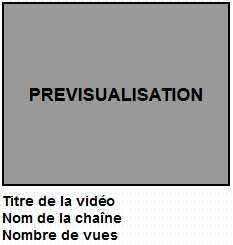
\includegraphics[width=0.2\textwidth]{../img/Miniature.png}
			\caption{Miniature}
			\label{Miniature}
		\end{figure}
		
		\subsection{Notification}
		Les notifications sont affichée sous cette forme
		\begin{figure}[h]
			\center
			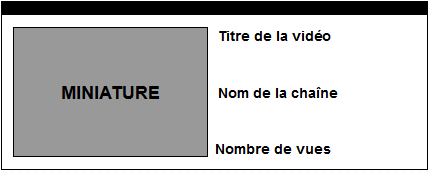
\includegraphics[width=0.4\textwidth]{../img/NotificationInterface.png}
			\caption{Interface notification}
			\label{notification}
		\end{figure}
		
		\subsection{Navigation}
		Les couleurs représentent les différentes fenêtres de l'application.
		
		\begin{figure}[h]
			\center
			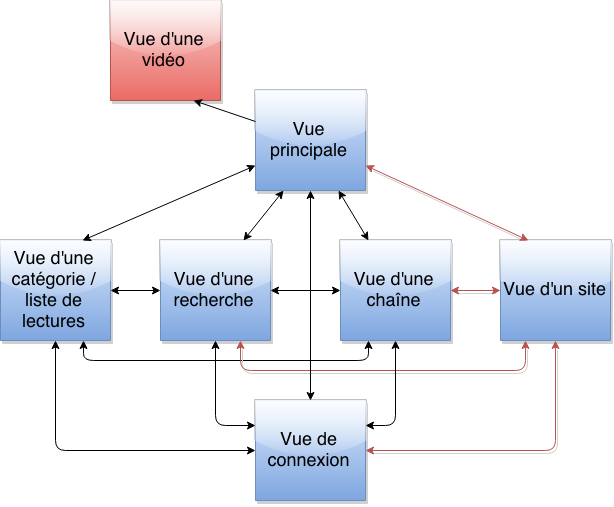
\includegraphics[width=0.8\textwidth]{../img/navigation.png}
			\caption{Navigation de l'application}
			\label{navigation}
		\end{figure}
		
		\subsection{Interface personnelle}
		Si l'utilisateur de l'application n'est connecté à aucun compte, le contenu de cette interface ce désactive sauf la partie 1 qui permet à l'utilisateur de se connecter avec ses différents comptes.
		\begin{figure}[h]
			\center
			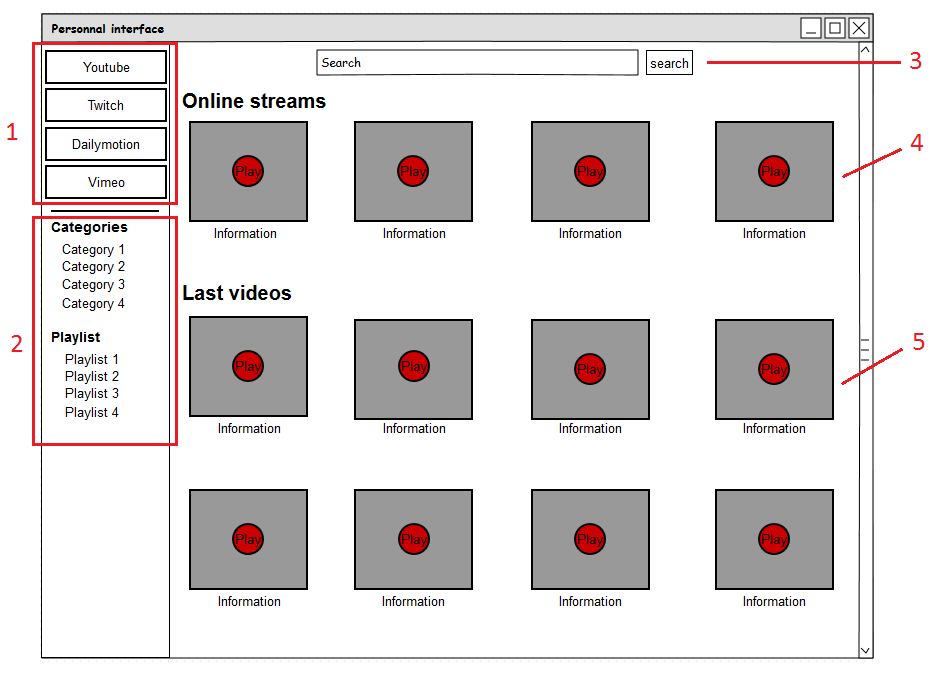
\includegraphics[width=1\textwidth]{../img/personnalInterfacenum.png}
			\caption{Interface personnel}
			\label{interfacepersonnel}
		\end{figure}
		
			\begin{enumerate}
				\item Boutons permettant d'accéder à l'interface concernant le site en question
				\item Liste des catégories et des listes de lecture et affiche le contenu dans l'interface
				\item Recherche de flux vidéo et affiche le résultat dans l'interface
				\item Liste des diffusions de vidéo en direct et ouvre une nouvelle interface pour voir le flux vidéo
				\item Liste des vidéos dernièrement sorties et ouvre une nouvelle interface pour voir le flux vidéo
			\end{enumerate}
		
		\newpage		
		
		\subsection{Interface des sites}
		L'interface des sites est commune pour tous les sites. Chaque site à une interface générique. 
		\begin{figure}[h]
			\center
			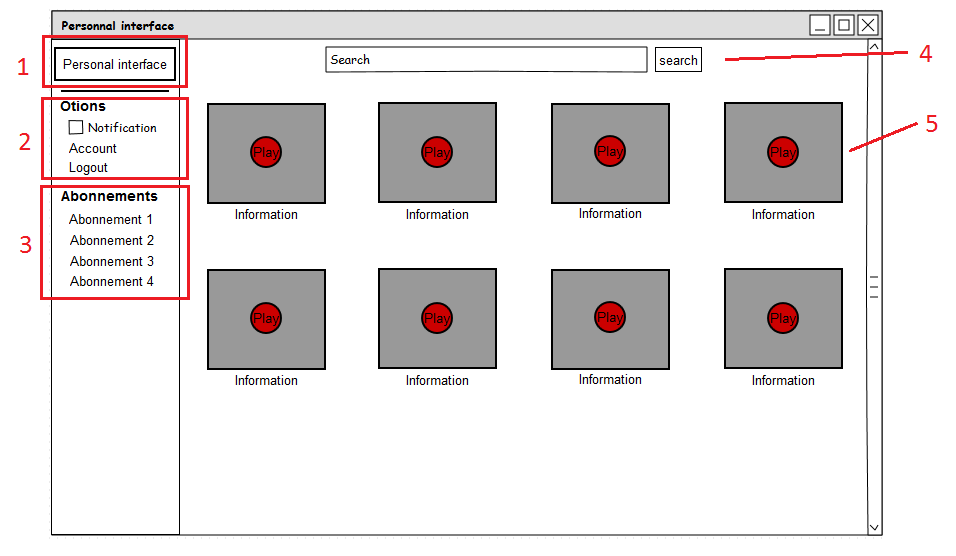
\includegraphics[width=1\textwidth]{../img/serviceInterfacenum.png}
			\caption{Interface des sites}
			\label{interfacesites}
		\end{figure}
		
		\begin{enumerate}
			\item Bouton permettant d'accéder à l'interface personnel
			\item Les options possibles concernant le compte de l'utilisateur
			\item La liste des abonnements / suivis 
			\item Recherche de flux vidéo et affiche le résultat dans l'interface
			\item Liste des flux vidéos
		\end{enumerate}

		\newpage

		\subsection{Interface vidéo}
		L'interface vidéo est générique, pour chaque vidéo de chaque site c'est la même interface. 
		\begin{figure}[h]
			\center
			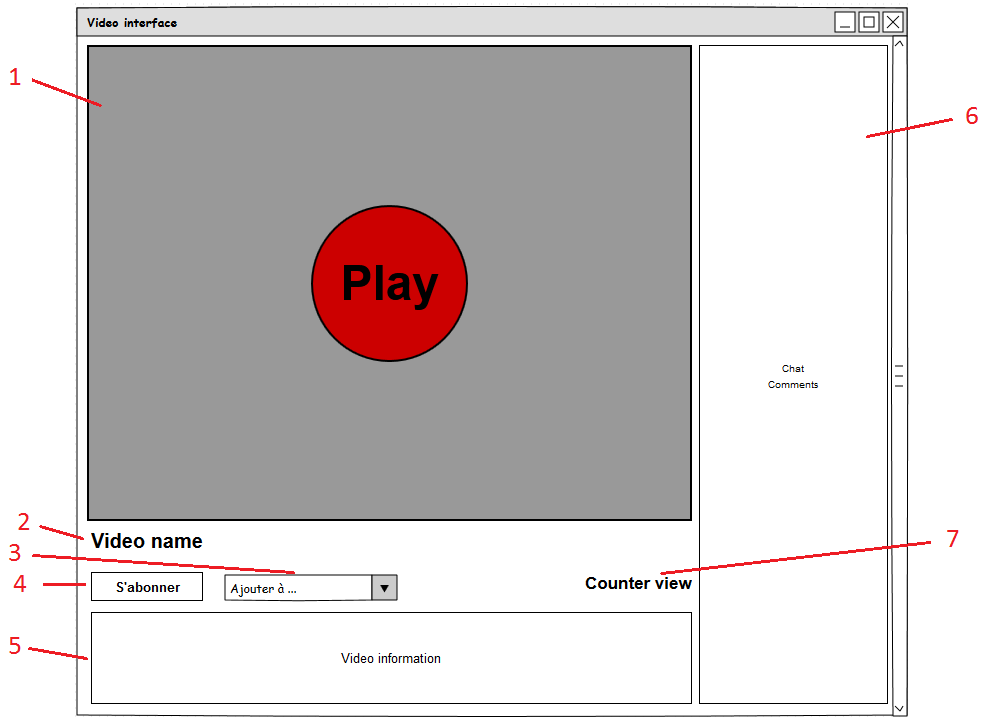
\includegraphics[width=1\textwidth]{../img/videoInterfacenum.png}
			\caption{Interface d'une vidéo}
			\label{interfacevideo}
		\end{figure}
		
		\begin{enumerate}
			\item Flux vidéo
			\item Nom de la vidéo
			\item Ajouter le flux vidéo à une catégorie ou liste de lecture
			\item S'abonner à l'auteur de la vidéo
			\item Informations concernant la vidéo
			\item \textit{Chat} ou espace commentaires
			\item Nombre de vues de la vidéo
		\end{enumerate}
		
		\newpage
		
		\subsection{Interface détail d'un compte}
		
		\begin{figure}[h]
			\center
			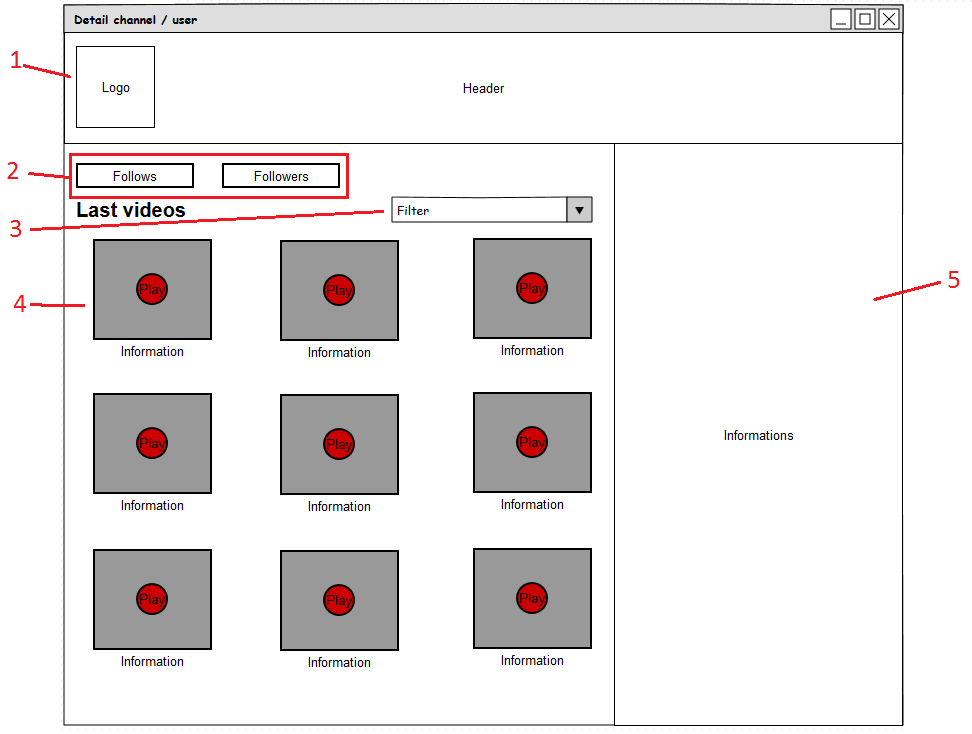
\includegraphics[width=1\textwidth]{../img/channelInterfacenum.png}
			\caption{Interface d'une chaîne / utilisateur}
			\label{interfacechannel}
		\end{figure}
		
		\begin{enumerate}
			\item Logo et bannière de la chaîne en question
			\item Bouton pour afficher les suivis et suiveurs de la chaîne
			\item Filtre sur les vidéos à afficher : Populaire, nouvelles etc ...
			\item Liste des flux vidéos
			\item Diverses informations concernant la chaîne
		\end{enumerate}
		
		\subsection{Interface de connexion}
		
		
\chapter{Analyse organique}
	\section{Généralité}
		\subsection{Langage en environnement de développement}
		L'application est développée en C\# sur Microsoft Visual Studio 2013. 
		
		\subsection{Format des fichiers et enregistrements}
		L'application stocke sa configuration sous forme de fichier. En effet, l'application a besoin d'enregistrer les catégories, listes de lecture ainsi que tout leurs contenu. Elle à également besoin d'enregistrer quelques configurations. C'est pour ça que j'utilise le format de fichier INI\footnote{Fichier de configuration} car il est très facile à manipuler. 
		
		\begin{figure}[h]
			\center
			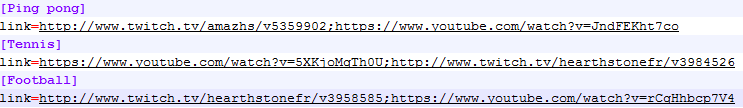
\includegraphics[width=0.7\textwidth]{../img/inifile.png}
			\caption{Exemple de fichier INI}
			\label{inifile}
		\end{figure}
		
		Pour plus de facilitée dans l'enregistrement des données, je crée deux fichiers INI : Category.ini et Playlist.ini
			
		\newpage
		
		\subsection{SVideo \& SChannel}
			Afin d'avoir un type générique pour traiter les vidéos de touts les sites de la même manière, j'ai créé deux structures. Elles contiennent toutes les informations commune de touts sites.
			
			SVideo : Structures pour les vidéos et vidéos en direct
			
			\begin{figure}[h]
				\center
				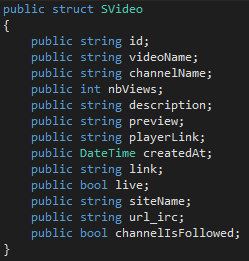
\includegraphics[width=0.4\textwidth]{../img/SVideo.png}
				\caption{Structure SVideo}
				\label{SVideo}
			\end{figure}
			
			SChannel : Structure pour les chaînes
			
			\begin{figure}[h]
				\center
				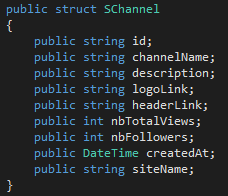
\includegraphics[width=0.4\textwidth]{../img/SChannel.png}
				\caption{Structure SChannel}
				\label{SChanel}
			\end{figure}
			
	\newpage
	\section{Conception}
		\subsection{Modèle}
			\subsubsection{StreamingSite}
			Pour pouvoir traiter les différents sites de la même manière, j'ai créer une classe de base qui sert de "modèle" aux classes des sites.
			Les classes de sites doivent contenir les mêmes méthodes que la classe de base.
			
			\begin{figure}[h]
				\center
				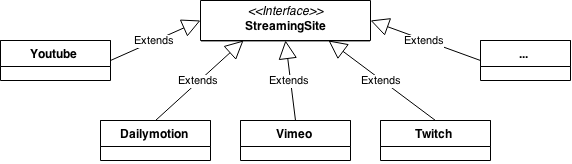
\includegraphics[width=1\textwidth]{../img/StreamingSite.png}
				\caption{Diagramme StreamingSite}
				\label{streaming site}
			\end{figure}
			
			Pour ajouter d'autres sites il faut juste créer une classe qui respecte la classe de base.
			Les méthodes commune à touts les sites sont virtuelles, en effet, étant donnée que pour chaque site les traitements ne sont pas les mêmes, il faut réécrire la méthode pour chaque site dans leurs classe respéctive.
			
			\begin{figure}[h]
				\center
				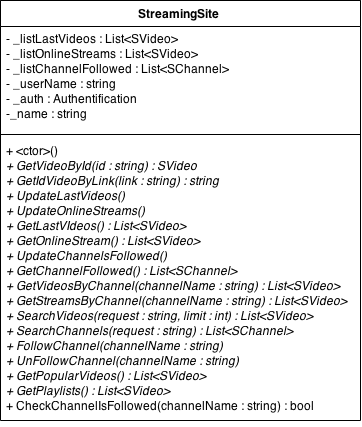
\includegraphics[width=0.4\textwidth]{../img/streamingsiteuml.png}
				\caption{StreamingSite table UML}
				\label{streaming site uml}
			\end{figure}
			
			\subsection{Catégorie et liste de lectures}
			Pour différencier les catégories et les liste de lectures j'ai créer une classe de base \textit{Container} qui contient toute les méthodes concernant les deux types de containeur.
			Étant donné que les liste de lectures sont des catégories avec une gestion de lecture en plus, j'ai crée une classe \textit{Playlist} qui contient uniquement les méthodes concernant les listes de lectures.
			
			Les vidéos sont stockée sous forme de liens, cela me permet de reconnaître de quel site est la vidéo. Ainsi, je peux récupérer les informations d'une vidéo grâce à l'id de la vidéo qui se trouve dans son lien.
				
			\begin{figure}[h]
				\center
				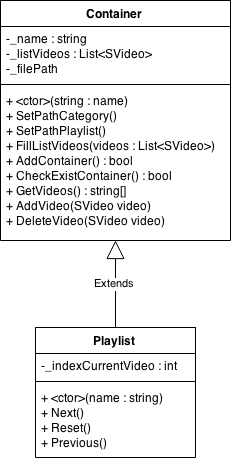
\includegraphics[width=0.3\textwidth]{../img/Container.png}
				\caption{Diagramme Container}
				\label{Container}
			\end{figure}
		
			\subsection{Authentification}
			L'authentification se fait au niveau du site, elle est différente pour chaque site.
			
			\begin{figure}[h]
				\center
				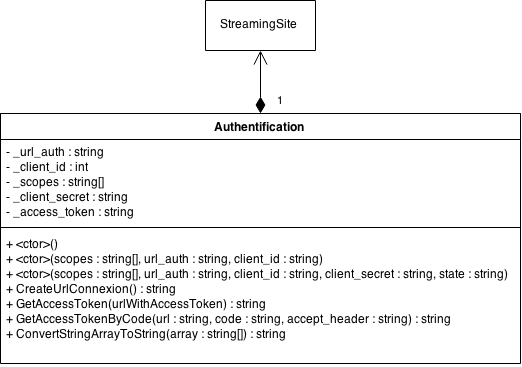
\includegraphics[width=0.7\textwidth]{../img/authuml.png}
				\caption{Authentification table uml}
				\label{authuml}
			\end{figure}
			
			
	\newpage
	\subsection{Global}
	
		\begin{figure}[h]
			\center
			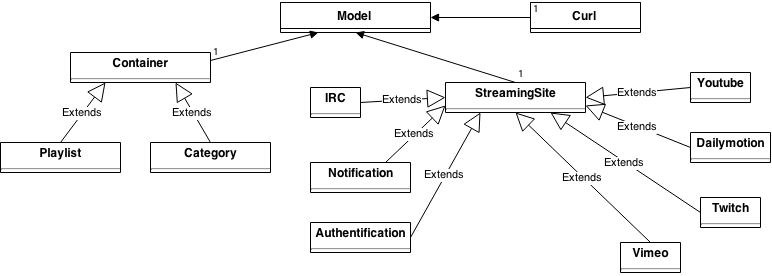
\includegraphics[width=1\textwidth]{../img/Model.png}
			\caption{Diagramme global}
			\label{Global}
		\end{figure}
			
	\newpage
	\section{Outil communautaire}
		\subsection{IRC}
		Le chat IRC a été réalisé grâce à la librairie mise à disposition sur GitHub "ChatSharp". Cette librairie sert à se connecter a un chat IRC ainsi que de recevoir les données envoyé sur le chat.
		La librairie "ChatSharp" offre des classes permettant de créer un utilisateur IRC ainsi qu'un client IRC. \\
		
		Afin de créer une connexion IRC il faut un nom d'utilisateur, celui du compte connecté. Un pseudonyme, je met le nom d'utilisateur. Il faut également un jeton d'accès qui permet de se connecter aux chats depuis l'extérieur.\\
		Ci-dessous les étapes d'une connexion à un chat IRC :
		
		\begin{figure}[h]
			\center
			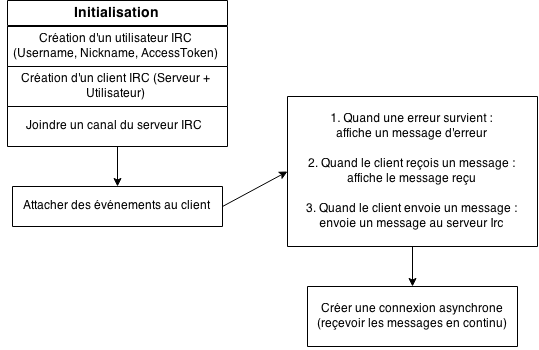
\includegraphics[width=0.8\textwidth]{../img/IrcChat.png}
			\caption{Étape de connexion à un chat IRC}
			\label{IrcChat}
		\end{figure}
		
		Les messages reçuent des événements sont affiché dans un TextBox.

	\newpage
	\section{Récupération des données}
		\subsection{Classes structure}
		Afin de récupérer les données reçues grâce aux API, j'ai créé des classes structures. En effet, ces classes ne sont composées que de propriétés et n'ont pas de méthodes. Chaque propriété est une donnée reçue suivant la demande envoyée.
		
		Pour spécifié que se sont des classes "structures" il faut spécifié la classe en \textit{[DataContract]} et les propriétés en \textit{[DataMember]}.
		
		\begin{figure}[h]
			\center
			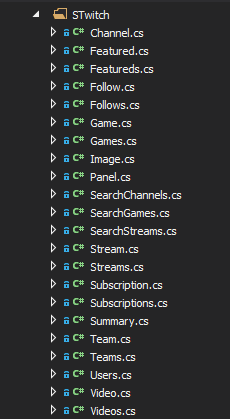
\includegraphics[width=0.3\textwidth]{../img/STwitch.png}
			\caption{Classes Twitch}
			\label{Twitch class}
		\end{figure}
		
		Ci-dessus, les classes "structures" du site Twitch. Il y a une liste de classes pour chaque site intégré à l'application. On peut trouver les différentes classes "structures" dans la documentation des différentes API.
		
		\newpage
		\subsection{Curl}
		Client URL Request Library est une interface en ligne de commande. Elle permet de récupérer des données d'une ressource accessible par réseau. On désigne la ressource à partir d'une URL.
		
		\begin{figure}[h]
			\center
			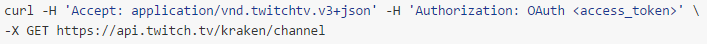
\includegraphics[width=1\textwidth]{../img/curl.png}
			\caption{Exemple de commande cURL}
			\label{cURL command}
		\end{figure}
		
		Ci-dessus, un exemple de récupération de données sur le site Twitch. La ressource désignée est "https://api.twitch.tv/kraken/channel".\\
		
		Il y a plusieurs type de requêtes :
		\begin{itemize}
			\item GET
			\item POST
			\item PUT
			\item DELETE
		\end{itemize}
		
		En C\#, afin de récupérer les données d'une ressource, j'utilise la classe proposée par le Framework .NET 4.5 \textbf{httpWebRequest}.\\		
		J'ai créé une fonction qui permet de récupérer la réponse d'une requête HTML :
		
		\begin{lstlisting}
		        /// <summary>
		        /// Send request and get response html
		        /// </summary>
		        /// <param name="urlRequest">request url</param>
		        /// <param name="p_method">method to use</param>
		        /// <param name="p_access_token">user access token</param>
		        /// <param name="acceptHeader">the accept header html</param>
		        /// <returns>HttpWebResponse</returns>
		        public static Stream SendRequest(string urlRequest, string p_method, string p_access_token, string acceptHeader)
		        {
			        //Create a new http request
			        var httpWebRequest = (HttpWebRequest)WebRequest.Create(urlRequest);
			        
			        //Init the http request
			        httpWebRequest.ContentType = "application/json";
			        httpWebRequest.Accept = acceptHeader;
			        httpWebRequest.Method = p_method;
			        httpWebRequest.Headers.Add("Authorization: OAuth " + p_access_token);
			        
			        if (p_method == "PUT")
				        httpWebRequest.ContentLength = 0;
			        
			        //Create a http response
			        Stream httpResponse = httpWebRequest.GetResponse().GetResponseStream();
			        
			        return httpResponse;
		        }
		\end{lstlisting}
		
		Il faut ensuite désérialiser cette réponse. Afin d’avoir une méthode qui renvoie le bon type suivant la ressource demandée, j’ai utilisé le type générique de C\#. C'est lors de l'appel de la méthode que l'on spécifie de quel type est la valeur de retour.
		
		\begin{lstlisting}
		/// <summary>
		/// Deserialize a http web response
		/// </summary>
		/// <typeparam name="T">Generic type</typeparam>
		/// <param name="jsonContent">content json</param>
		/// <returns>the object deserialized</returns>
		public static T Deserialize<T>(Stream jsonContent)
		{
			var httpResponse = jsonContent;
			
			//Read the response
			using (var streamReader = new StreamReader(httpResponse))
			{
				//Add to the generics variable the result
				T answer = JsonConvert.DeserializeObject<T>(streamReader.ReadToEnd());
				return answer;
			}
		}
		\end{lstlisting}
		
	\newpage
	\section{Authentification}
	L'authentification se fait grâce au protocole OAuth2[AJOUTER REFERENCE]. Pour rendre l'authentification générique il faut utiliser le même type d'autorisation. Dans notre cas, le problème est que pas tout les sites utilisent le type d'autorisation implicite.\\
	C'est pour cela que j'ai créé une classe permettant la connexion implicite ainsi que la connexion par autorisation de flux.
	
	\subsection{Générique}
	Je rencontre un problème pour la connexion générique, en effet, afin de pouvoir utiliser le protocole OAuth2, il faut que j'utilise ASP.NET. 
	Afin d'éviter l'utilisation d'ASP.NET, je n'utilise pas moi même le protocole OAuth2 mais je le sous-traitre aux API.\\
	Je procède de cette manière :
	
			\begin{figure}[h]
				\center
				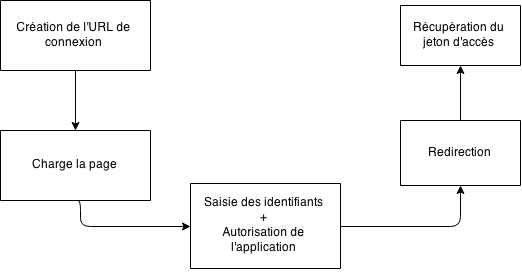
\includegraphics[width=0.7\textwidth]{../img/auth.png}
				\caption{Authentification}
				\label{authentification}
			\end{figure}
	
	
	La création de l'URL de connexion se fait par rapport au site sur lequel l'utilisateur veut se connecter. En effet, les services proposent une page Web permettant à un utilisateur de se connecter à son compte sur une application ainsi que de l'autoriser.
	L'url de cette page Web est composée comme suit : \\
	
	\textit{https://[url de l'api]?response\_type=token\&client\_id="[id de l'application]"\& redirect\_uri="[page de redirection]"\&scope="[Liste des droits]"}\\
	
	Le client\_id est l'id que donne le service chez qui j'ai enregistrer mon application, il varie pour chaque site. 
	La page de redirection sert uniquement à récupérer le jeton d'accès dans le lien, en effet si l'utilisateur saisi correctement ses identifiants il sera redirigé sur cette page. Il doit également accepter l'utilisation de son compte sur mon application.

	\subsection{Connexion automatique}
	La connexion automatique est la connexion aux différents comptes de l'utilisateur lors de l'ouverture de l'application. Malheureusement, c'est techniquement impossible, en effet, le faits de devoir passer de toute façon par une page web fais que l'on ne peut pas remplir automatiquement les champs d'identifiants.
	
	Le navigateur intégrer dans Visual Studio utilise Internet Explorer, et donc prends en compte les cookies. Cela ne remplace pas la connexion automatique mais l'utilisateur passe moins de temps à se connecter car les identifiants sont déjà enregistré, il suffit juste de cliquer sur un bouton pour valider la connexion.

	\newpage
	
	\section{Notification}
	
	Afin d'être notifié lorsqu'une vidéo sort ou lorsque une diffusion de flux vidéo en direct commence, je compare deux listes. La première contient les vidéos ACTUELLEMENT sorties et les diffusions en direct, la deuxième va récupérer depuis une requête la liste des vidéos sorties. \\
	Chaque X secondes on compare les deux listes pour voir si il y a eu une vidéo qui est en plus dans la deuxième liste.
	
	\begin{figure}[h]
		\center
		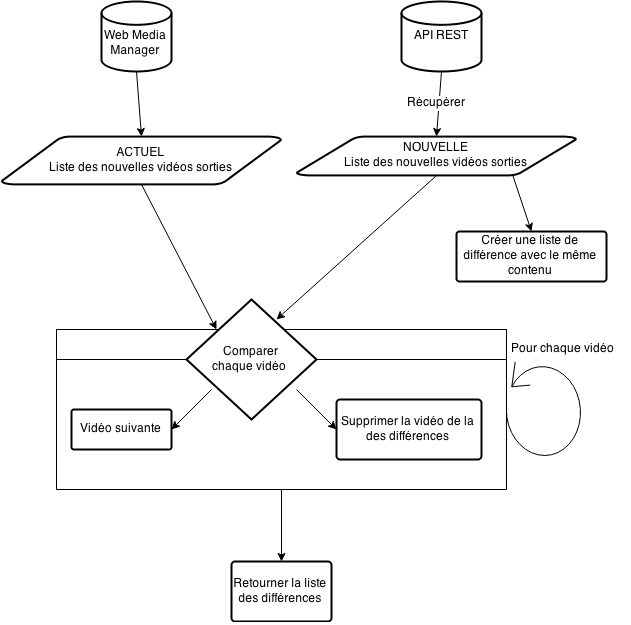
\includegraphics[width=0.8\textwidth]{../img/notification.png}
		\caption{Notification}
		\label{checkNotif}
	\end{figure}
	
	\newpage
	\section{Affichage}	
		\subsection{Flux vidéo}
		Les flux vidéos sont affiché grâce au composant de base proposé par .NET : WebBrowser. En effet, tout les sites proposent un lien afin d'avoir uniquement le lecteur vidéo.
		J'ai choisi cette solution car chaque lecteur est différent et ont donc certaine fonctionnalités le sont aussi.
		
		\subsection{Chat IRC}
		Comme dis plus haut, les messages du chat sont affichés dans un TextBox. Afin de pouvoir y afficher depuis un événements j'ai du créer un autre processus.
		
		
		\subsection{Notification}
		Le composant externe "PopopNotifier" a été utilisé pour afficher un pop-up lorsqu’une nouvelle
		diffusion commence. Ce composant vient du web : http://www.codeproject.com/Articles/
		277584/Notification-Window.
		
		TODO : METTRE IMAGE
		
		Pour rendre le composant plus attrayant et adapté à mon interface homme-machine, j’ai modifié
		certains éléments graphiques à l'interne du composant.
		Les différentes informations affichées : Nom de la vidéo ; nom de la chaîne ; nombre de vues	
		
	
\chapter{Tests}
	\section{Tests fonctionnel}
	\section{Tests unitaire}
	
\chapter{Conclusions}

\chapter{Annexes}
	\section{Planning}
	\subsection{Initial}
	
	\begin{ganttchart}[hgrid,vgrid,x unit=6mm,y unit chart=6mm,group left shift=0,group right shift=0,group peaks tip position=0,group peaks height=.4]{1}{14}
		\gantttitle{\textbf{Avril}}{14}\ganttnewline
		\gantttitlelist{13,14,15,16,17,20,21,22,23,24,27,28,29,30}{1}\ganttnewline
		\ganttbar[bar height=.6, bar top shift=.2, bar/.append style={fill=green}]{Étude d'opportunité}{1}{1}\ganttnewline
		\ganttbar[bar height=.6, bar top shift=.2, bar/.append style={fill=green}]{Analyse fonctionnelle}{2}{4}\ganttnewline
		\ganttbar[bar height=.6, bar top shift=.2, bar/.append style={fill=green}]{Analyse organique}{5}{8}\ganttnewline
		\ganttbar[bar height=.6, bar top shift=.2, bar/.append style={fill=red}]{Développement}{9}{14}
	\end{ganttchart}
	
	\begin{ganttchart}[hgrid,vgrid,x unit=5mm,y unit chart=6mm,group left shift=0,group right shift=0,group peaks tip position=0,group peaks height=.4]{1}{18}
		\gantttitle{\textbf{Mai}}{18}\ganttnewline
		\gantttitlelist{4,5,6,7,8,11,12,13,15,18,19,20,21,22,26,27,28,29}{1}\ganttnewline
		\ganttbar[bar height=.6, bar top shift=.2, bar/.append style={fill=red}]{Développement}{1}{14}\ganttnewline
		\ganttbar[bar height=.6, bar top shift=.2, bar/.append style={fill=yellow}]{Tests}{15}{16}\ganttnewline
		\ganttbar[bar height=.6, bar top shift=.2, bar/.append style={fill=green}]{Conclusions/Bilan}{17}{18}
	\end{ganttchart}
	
	\subsection{Final}

\listoffigures

\end{document}
